%%%%%%%% ICML 2018 EXAMPLE LATEX SUBMISSION FILE %%%%%%%%%%%%%%%%%

\documentclass{article}

% Recommended, but optional, packages for figures and better typesetting:
\usepackage{amsmath}
\usepackage{microtype}
\usepackage{graphicx}
\usepackage{subfigure}
\usepackage{booktabs} % for professional tables
\usepackage{amssymb}
\usepackage{multicol}
\usepackage{epstopdf}
% hyperref makes hyperlinks in the resulting PDF.
% If your build breaks (sometimes temporarily if a hyperlink spans a page)
% please comment out the following usepackage line and replace
% \usepackage{icml2018} with \usepackage[nohyperref]{icml2018} above.
\usepackage{hyperref}

% Attempt to make hyperref and algorithmic work together better:
\newcommand{\theHalgorithm}{\arabic{algorithm}}

% Use the following line for the initial blind version submitted for review:
\usepackage{example/icml2018}

% If accepted, instead use the following line for the camera-ready submission:
%\usepackage[accepted]{icml2018}

% The \icmltitle you define below is probably too long as a header.
% Therefore, a short form for the running title is supplied here:
\icmltitlerunning{Bayesian prediction of intensity rates from multivariate point processes}

\begin{document}

\twocolumn[
\icmltitle{Probabilistic forecast of influenza from genetic and count data}

% It is OKAY to include author information, even for blind
% submissions: the style file will automatically remove it for you
% unless you've provided the [accepted] option to the icml2018
% package.

% List of affiliations: The first argument should be a (short)
% identifier you will use later to specify author affiliations
% Academic affiliations should list Department, University, City, Region, Country
% Industry affiliations should list Company, City, Region, Country

% You can specify symbols, otherwise they are numbered in order.
% Ideally, you should not use this facility. Affiliations will be numbered
% in order of appearance and this is the preferred way.
\icmlsetsymbol{equal}{*}

\begin{icmlauthorlist}
\icmlauthor{Aeiau Zzzz}{equal,to}
\icmlauthor{Bauiu C.~Yyyy}{equal,to,goo}
\icmlauthor{Cieua Vvvvv}{goo}
\icmlauthor{Iaesut Saoeu}{ed}
\icmlauthor{Fiuea Rrrr}{to}
\icmlauthor{Tateu H.~Yasehe}{ed,to,goo}
\icmlauthor{Aaoeu Iasoh}{goo}
\icmlauthor{Buiui Eueu}{ed}
\icmlauthor{Aeuia Zzzz}{ed}
\icmlauthor{Bieea C.~Yyyy}{to,goo}
\icmlauthor{Teoau Xxxx}{ed}
\icmlauthor{Eee Pppp}{ed}
\end{icmlauthorlist}

\icmlaffiliation{to}{Department of Computation, University of Torontoland, Torontoland, Canada}
\icmlaffiliation{goo}{Googol ShallowMind, New London, Michigan, USA}
\icmlaffiliation{ed}{School of Computation, University of Edenborrow, Edenborrow, United Kingdom}

\icmlcorrespondingauthor{Cieua Vvvvv}{c.vvvvv@googol.com}
\icmlcorrespondingauthor{Eee Pppp}{ep@eden.co.uk}

% You may provide any keywords that you
% find helpful for describing your paper; these are used to populate
% the "keywords" metadata in the PDF but will not be shown in the document
\icmlkeywords{Machine Learning, ICML}

\vskip 0.3in
]

% this must go after the closing bracket ] following \twocolumn[ ...

% This command actually creates the footnote in the first column
% listing the affiliations and the copyright notice.
% The command takes one argument, which is text to display at the start of the footnote.
% The \icmlEqualContribution command is standard text for equal contribution.
% Remove it (just {}) if you do not need this facility.

%\printAffiliationsAndNotice{}  % leave blank if no need to mention equal contribution
\printAffiliationsAndNotice{\icmlEqualContribution} % otherwise use the standard text.

\begin{abstract} 
\end{abstract}

\section{Introduction}

\section{Methods}
\begin{figure}[h]
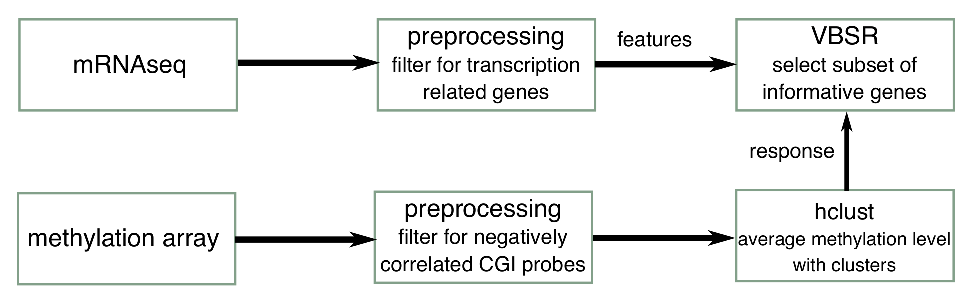
\includegraphics[width=0.5\textwidth]{../figs/flowChart}
\caption{\textbf{Pipeline}}
\end{figure}
\subsection{data preprocessing}
TCGA Level 3 mRNAseq and DNA methylation data (HumanMethylation450 arrays) was downloaded from Broad TCGA GDAC site for LAML, SKCM and HNSC. mRNAseq probes with missing values were removed. We queried the GO terms (molecular function and biological process) based on the HUGO symbol of the probes and kept only probes that contain keywords related to transcription and methylation as our feature matrix.   

Methylation array data was filtered to remove probes that are on chromosome X and Y and have missing values. Probes with UCSC RefGene group annotation as TSS 1500 and located within UCSC CpG island annotation were selected. The correlation between the Beta value of filtered methylation probes and RSEM level of the corresponding genes in mRNAseq data were computed and significant methylation probes was filtered with FDR adjusted p-value (FDR < 0.1) of 0.05. The resulting probes were clustered using hierarchical clustering with euclidean distance using Ward's method. 20 clusters were set as the cutoff for assigning cluster membership. The average methylation level within the cluster of each patient was computed as the response vector. 

\subsection{variational Bayesian spike regression}
variational Bayesian spike regression (VBSR) \cite{logsdon2012novel} is a Bayesian approximation of best subset selection. We used VBSR to select subset of informative mRNAseq probes that best explain the observed pattern of methylation level across patients out of all possible subset. VBSR approaches the problem by using a variational Bayes approximation that probabilistically models the inclusion of any probes in the regression model. The p-value on the estimated value of penalized regression coefficient were computed and significant probes were extracted at FDR adjusted p-value (FDR < 0.1) of 0.05. R package \texttt{vbsr} was used. 

\subsection{Geneset analysis of methylation clusters}
The enrichment of biological processes in each methylation clusters were examined by comparing to pre-defined genesets on MSigDB by hypergeometric test. 

\section{Results}

\section{Discussion}

\bibliography{main}
\bibliographystyle{example/icml2018}

\end{document}
